\section{Характеристика объекта автоматизации}


\subsection{Общее описание}

Объектом автоматизации является ролевая система Dungeons \& Dragons 3.5 редакции, а также игровой процесс, проводимый с использованием данной системы.

Суть любой ролевой системы в математическом обеспечении процесса игры. Наиболее часто такие системы применяются для проверки успешности действия или определения результата этого действия, однако этим использование ролевой системы в игровом процессе не ограничено. 

В качестве базовой функции ролевой системы можно обозначить описание отдельных аспектов игры (таких, например, как характеристики персонажа), которые используются как при расчете каких-либо действий, так и для описания (например, <<крепкий стол>> может иметь прочность равную десяти, в то время как <<хлипкий стол>> может иметь прочность, равную 3).

Для определения параметров в процессе игры (таких, например, как успешность некоторого действия) используются генераторы случайных чисел. В качестве таких генераторов используется набор игральных костей.

Игровой процесс, проводимый в соответствии с правилами ролевой системы Dungeons \& Dragons, включает в себя несколько стадий и определяет роли участников в данном процессе.

Для каждой игры определены две основные роли: игрок и мастер. Игрок~--- тот, кто участвует в процессе игры через управление персонажем. Первая задача, стоящая перед игроком~--- создание персонажа. Для этого игрок определяет характер и основные параметры персонажа, которые потом будут использоваться в игре. Основная задача игрока, следующая за созданием персонажа~--- непосредственно игра, то есть управление персонажем. Для этого в процессе игры игрок обозначает действия, которые пытается совершить его персонаж, после чего в зависимости от типа действия определяет успешность этого действия с помощью бросков игральных костей.

В игре может участвовать от одного до нескольких игроков. Число игроков является произвольным и не регламентировано правилами. Группа игроков, участвующих в одной игре называется партией.

Мастер игры определяет сценарий и основные параметры игры, в т.ч. игровой сеттинг, время и место событий. Для каждой игры нужен только один мастер. В задачи мастера входит управление процессом игры, координирование действий игроков. Также в задачи мастера входит определение адекватности действий игроков сеттингу и правилам, помощь в разрешении неясных или конфликтных ситуаций.

Каждая отдельно взятая игра характеризуется целью, которую в ходе этой игры необходимо выполнить. Достижение цели проходит в рамках игровой кампании. Длительность кампании правилами не регламентируется и, в зависимости от цели, может быть от одного-двух дней до нескольких лет.

Кампания состоит из игровых сессий. Игровая сессия — это отрезок времени, в пределах которого ведётся игра. В одной кампании может быть от одной до нескольких сессий. Каждая сессия в среднем длится от двух до десяти часов. После каждой игровой сессии мастер игры определяет предварительные результаты и фиксирует текущее состояние внутриигрового мира.


\subsection{Структура и принципы функционирования}

Игра с использованием ролевой системы \dnd включает в себя следующие процессы:
\begin{enumerate}
\item Подготовка к игре\\
Ролевая система \dnd является достаточно сложной и гибкой как с алгоритмической так и с концептуальной точки зрения. По этой причине процесс подготовки к игре является важным этапом и включает в себя несколько подпроцессов:
\begin{enumerate}
\item Создание сценария игры\\
Этот подпроцесс осуществляется мастером игры. В ходе данного подпроцесса создаётся идея игры, описание, создаются локации, генерируются персонажы. Немаловажным является определение начальных параметров, которые определяют сложность игры.
\item Создание персонажа\\
Данный подпроцесс осуществляется каждым из игроков. В ходе данного процесса игрок, на основе выданных мастером данных, создаёт концепцию персонажа, на основе которой затем подбирает параметры в соответствии с правилами игры и сеттингом.
\end{enumerate}
\item Игра\\
Игра состоит из нескольких сессий. В ходе сессии игроки совершают внутриигровые действия, общаются, производят локальные расчёты. Каждое действие в игре совершается в соответствиями с правилами игры, однако, если какое-то действие в правилах не описано, его результат определяется мастером. В некоторых случаях каждое совершаемое действие записывается в протокол сессии.

В ходе первой сессии следует выделить особый подпроцесс: расчёты. Так как многие расчёты следует провести под руководством мастера, эти расчёты невозможно включить в этап <<подготовка к игре>>.
\item Определение результатов игры\\
Подведение итогов игры является важным этапом как для мастера, так и для игроков.

В процессе определения результатов игры делаются выводы о качестве игрового процесса, обращается внимание на совершённые ошибки и недочёты для дальнейшего улучшения игрового процесса. Также в ходе подведения итогов определяется непосредственное завершение сценария, мастером игры частично описывается дальнейшая <<судьба>> персонажей, определяется, чего смогли достичь игроки за данную игру.

Немаловажным подпроцессом является составление отчёта. Данный отчёт должен содержать в себе как выводы относительно игрового процесса (качество игры, описание основных проблем), так и описание внутриигровых достижений. Данный отчёт может быть использован для восстановления состояния другой игры в том случае, если она будет основана на том же сценарии (например, будет являться продолжением).
\end{enumerate}

%%%%%%%%%%%%%%%%%%%%%%%%%%%%%%%%%%%%%%%%

В игровом процессе выполняются следующие операции по сбору и обработке информации:
\begin{enumerate}
\item Обмен персональными данными\\
Для участия в игре и возможности взаимодействия мастер и игроки обмениваются именами, номерами телефонов и адресами электронной почт
ы.
\item Начальные параметры\\
При создании материалов для игры мастер должен выбрать начальные параметры, такие как сеттинг, стартовый уровень, ограничения на параметры персонажа и пр. Все данные, полученные на этом этапе, передаются игрокам для создания персонажей.

\item Создание игрового окружения\\
На основании начальных параметров мастер создаёт описание локаций, ключевых событий и НИП. Часть этой информации может быть выдана игрокам для создания более подходящих персонажей.
\item Создание персонажей\\
После того, как выбраны начальные параметры, они передаются игрокам для создания персонажей. При создании персонажей игроки, используя полученную от мастера информацию, создают концепцию и описание персонажа. Затем на основе этих данных а также игровых руководств выбираются раса и класс. После этого используются игральные кости для генерации параметров и проводятся расчёты. Вся информация заносится в лист персонажа.
\item Проверка листов персонажей\\
После того, как расчёты проведены, игроки передают мастеру листы персонажа (или их копии) для проверки. В том случае, если в листах персонажа содержатся ошибки, листы передаются игрокам на доработку.
\item Обмен информацией во время игры\\
На основе сгенерированной информации начинается игровой процесс. На этом этапе происходит обмен внутриигровой информацией между мастером и игроками. В ходе игры могут изменяться данные, указанные в листах персонажей. Также могут записываться протоколы игр, составляться отчёты о проведённых сессиях. В отчёты и протоколы могут входить как общее описание, так и полные записи действий игроков и мастера.
\item Завершение игры\\
При завершении игры может создаваться общеигровой отчёт. Все отчёты и протоколы передаются ответственному лицу (в качестве которого чаще всего выступает мастер) на архивацию.
\end{enumerate}


\subsection{Существующая информационная система и её недостатки}

Далее представлены диаграммы, описывающие процессы в текущей информационной системе.

\begin{figure}[h]
\center{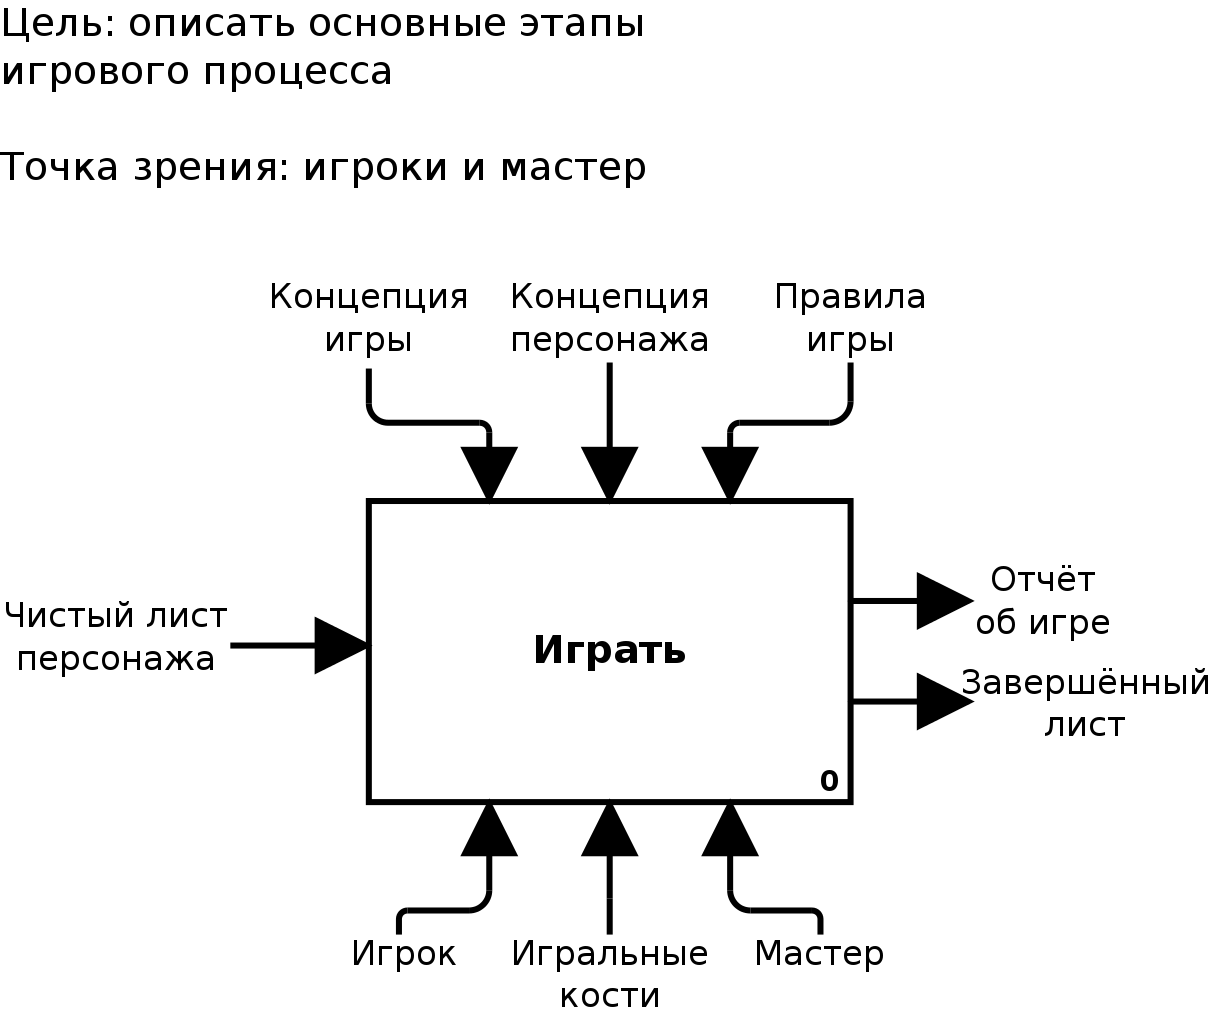
\includegraphics[width=1\linewidth]{images/current_idef/Context.png}}
\caption{Контекстная диаграмма исходной информационной системы}
\label{ris:current_context_diagram}
\end{figure}

\begin{figure}[h]
\center{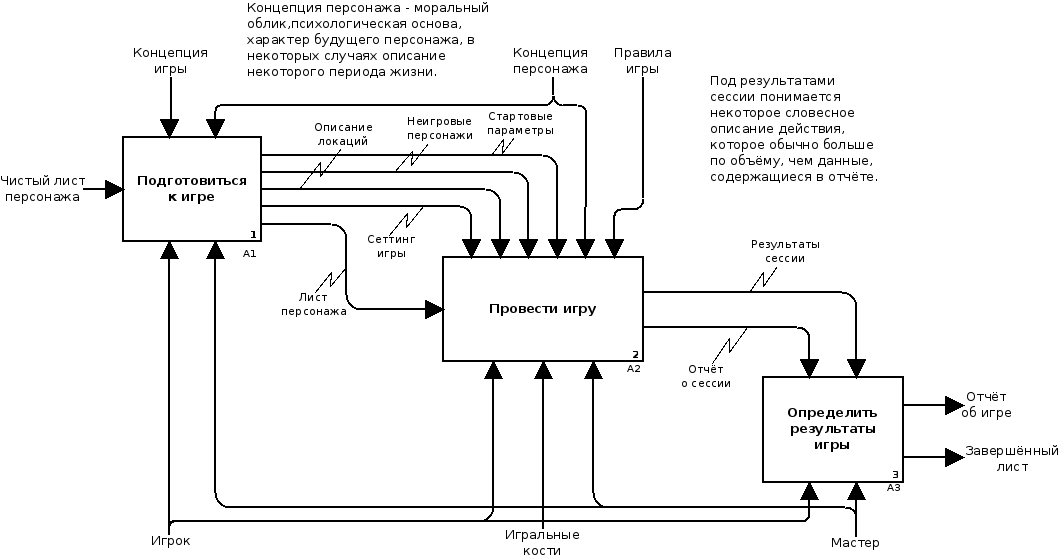
\includegraphics[width=1\linewidth]{images/current_idef/A0.png}}
\caption{Диаграмма A0 исходной информационной системы: описание процесса <<Играть>>}
\label{ris:current_a0_diagram}
\end{figure}

\begin{figure}[h]
\center{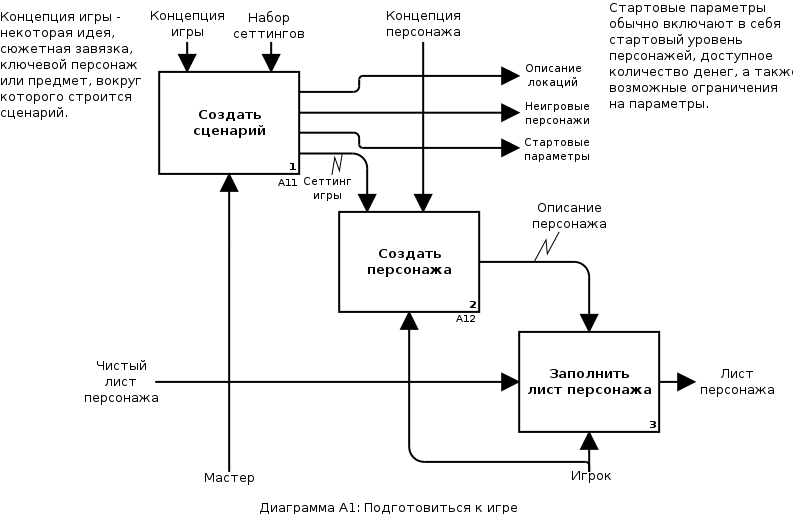
\includegraphics[width=1\linewidth]{images/current_idef/A1.png}}
\caption{Диаграмма A1 исходной информационной системы: описание процесса <<Подготовиться к игре>>}
\label{ris:current_a1_diagram}
\end{figure}

\begin{figure}[h]
\center{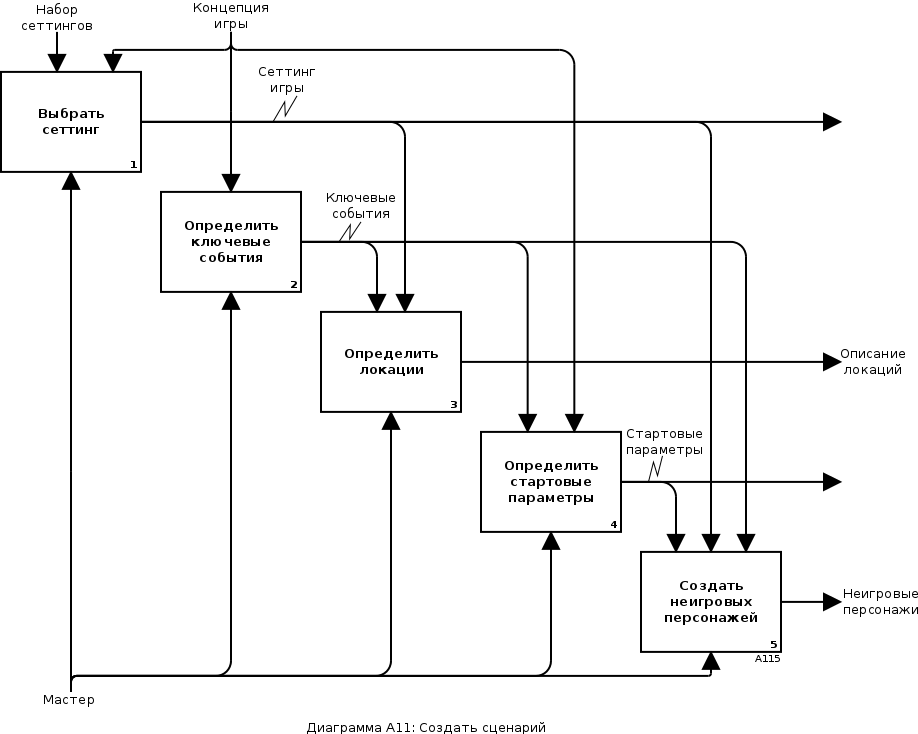
\includegraphics[width=1\linewidth]{images/current_idef/A11.png}}
\caption{Диаграмма A11 исходной информационной системы: описание процесса <<Создать сценарий>>}
\label{ris:current_a11_diagram}
\end{figure}

\begin{figure}[h]
\center{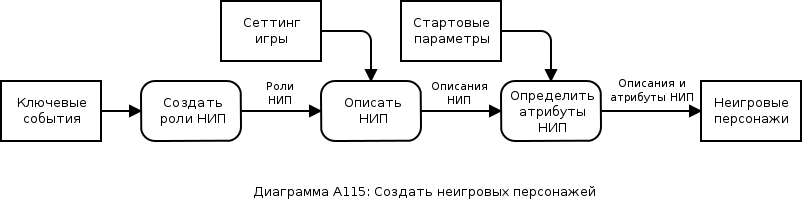
\includegraphics[width=1\linewidth]{images/current_idef/A115.png}}
\caption{Диаграмма A115 исходной информационной системы: описание процесса <<Создать неигровых персонажей>>}
\label{ris:current_a115_diagram}
\end{figure}

\begin{figure}[h]
\center{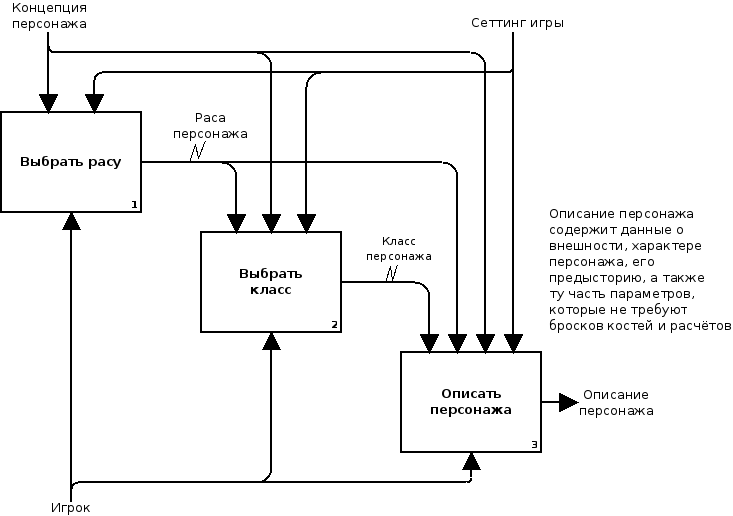
\includegraphics[width=1\linewidth]{images/current_idef/A12.png}}
\caption{Диаграмма A12 исходной информационной системы: описание процесса <<Создать персонажа>>}
\label{ris:current_a12_diagram}
\end{figure}

\begin{figure}[h]
\center{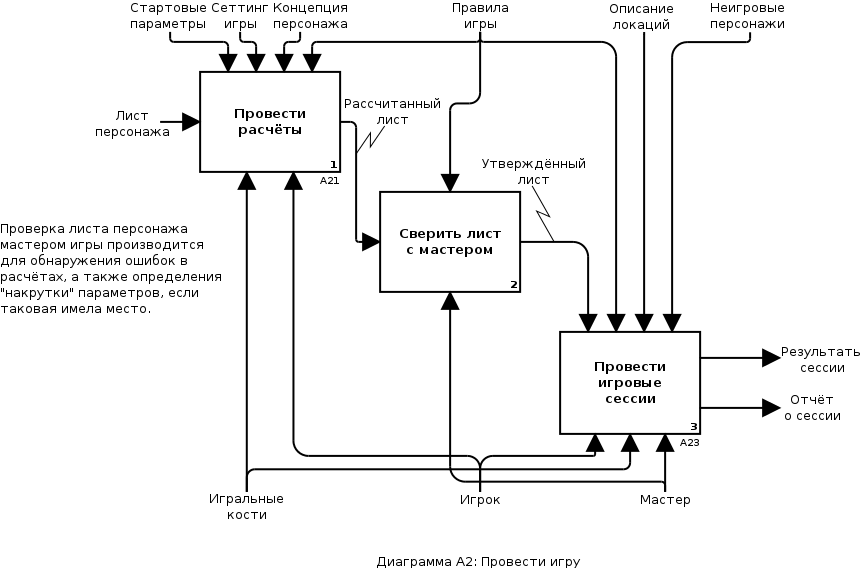
\includegraphics[width=1\linewidth]{images/current_idef/A2.png}}
\caption{Диаграмма A2 исходной информационной системы: описание процесса <<Провести игру>>}
\label{ris:current_a2_diagram}
\end{figure}

\begin{figure}[h]
\center{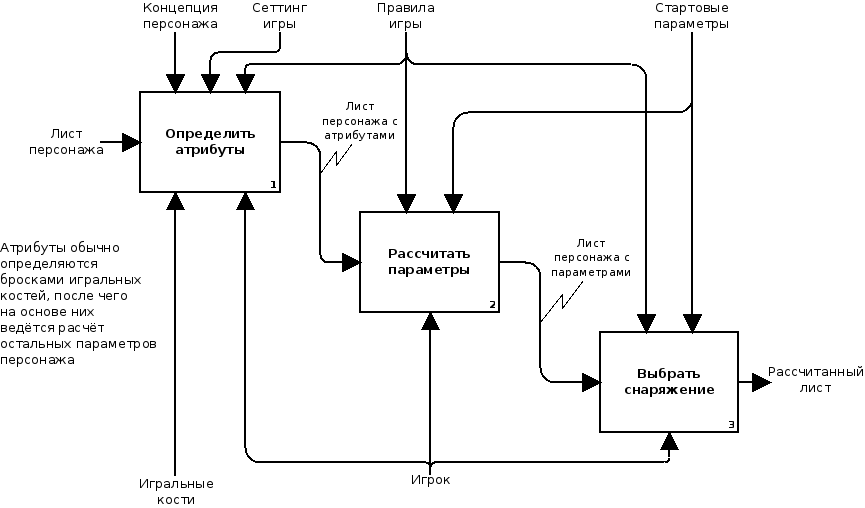
\includegraphics[width=1\linewidth]{images/current_idef/A21.png}}
\caption{Диаграмма A21 исходной информационной системы: описание процесса <<Провести расчёты>>}
\label{ris:current_a21_diagram}
\end{figure}

\begin{landscape}
  \vspace*{\fill}
  \begin{figure}[h]
  \center{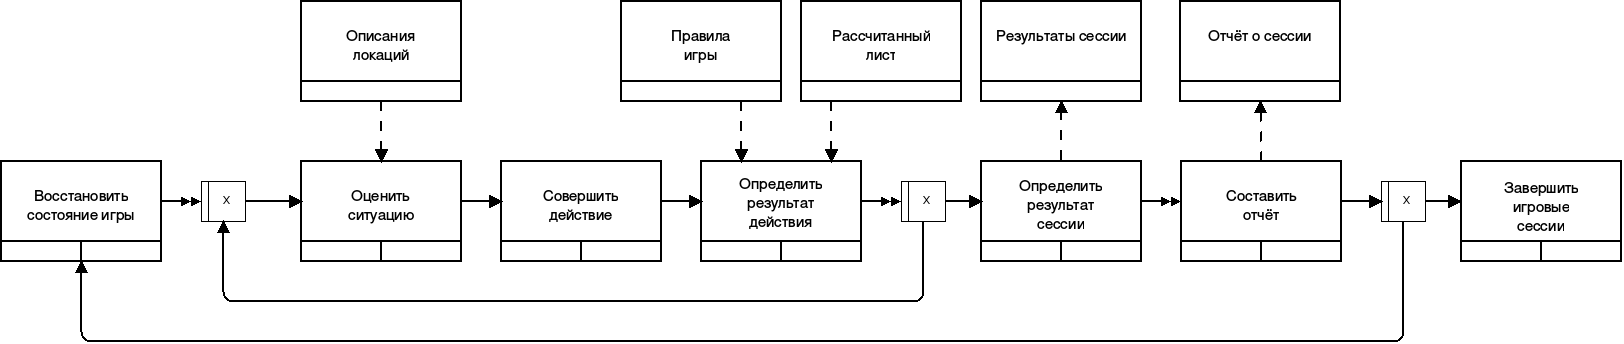
\includegraphics[width=1\linewidth]{images/current_idef/A22.png}}
  \caption{Диаграмма A22 исходной информационной системы: описание процесса <<Провести игровые сессии>>}
  \label{ris:current_a22_diagram}
  \end{figure}
  
\end{landscape}

\begin{figure}[h]
\center{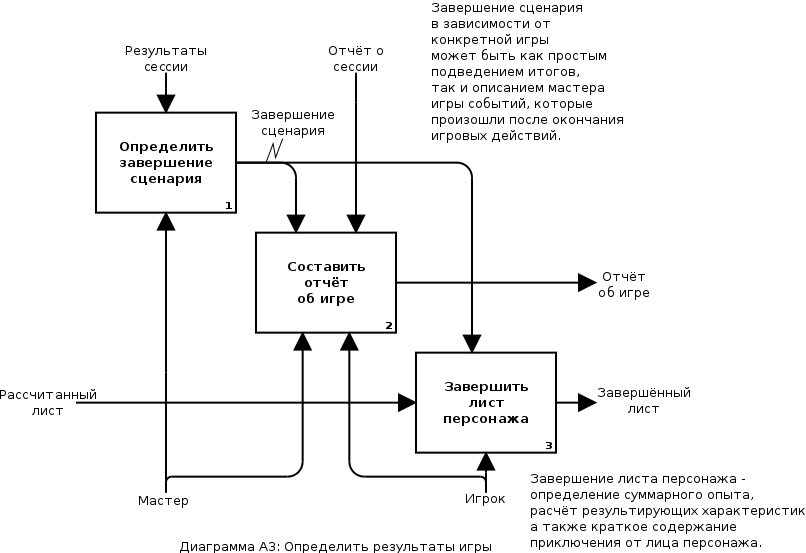
\includegraphics[width=1\linewidth]{images/current_idef/A3.png}}
\caption{Диаграмма A3 исходной информационной системы: описание процесса <<Определить результаты игры>>}
\label{ris:current_a21_diagram}
\end{figure}


Основными недостатками существующей информационной системы являются:
\begin{enumerate}
\item \textbf{Отсутствие автоматизации расчётов}\\
Игровой процесс с использованием ролевой системы \dnd\ включает в себя большое количество расчётов. Исходная модель не предоставляет специализированных средств для их автоматизации, что приводит к большим затратам времени --- от 30\% до 60\% времени обычно занимают расчёты.
\item \textbf{Отсутствие специализированного средства обмена информацией}\\
Для игры с использованием \dnd\ необходим обмен информацией --- как во время игровой сессии так и между сессиями. Обычно этот обмен осуществляется с помощью средств связи или сторонних информационных ресурсов (в т.ч. социальных сетей). Такие способы неэффективны, так как они не позволяют в удобном формате обмениваться специфичной информцией, такой как листы персонажей.
\item \textbf{Отсутствие централизованного средства хранения информации}\\
\dnd\ является набором правил и описаний. Обычно распространение информации происходит с помощью бумажных носителей --- книг и журналов. Количество книг, используемых для игры может быть значительным, а поиск информации в них может занимать длительное время.
\end{enumerate}


\subsection{Анализ аналогичных разработок}
\subsubsection{\href{http://www.wizards.com/dnd/Tool.aspx?x=dnd/4new/tool/adventuretools}{Dungeons \& Dragons Insider Adventure Tools}}
Данное средство автоматизации игрового процесса предоставляется официальным разработчиком игровой системы \dnd 4 редакции. Оно предоставляется всем подписчикам \href{http://www.wizards.com/dnd}{специализированного ресурса}.

\href{http://www.wizards.com/dnd/Tool.aspx?x=dnd/4new/tool/adventuretools}{Dungeons \& Dragons Insider Adventure Tools} предоставляет следующие возможности:
\begin{enumerate}
\item Автоматизированное создание персонажа
\item Генерация способностей персонажа
\item Генерация имён персонажей
\item Генерация монстров
\item Просмотр правил игры
\end{enumerate}


\subsection{Актуальность проводимой разработки}







